\documentclass[12pt]{article}

\usepackage{../gongkechuang}

\title{EI313-\texttt{libvirt} API}

\begin{document}

\maketitle

\section{Introduction}

In what follows, we explore the API provided by \texttt{libvirt} and use it to get a set of parameters in the virtual machine, such as ID, name, maximum memory, and number of virtual CPUs.

\texttt{libvirt} organizes virtual machines by domains. The next section covers how to connect to \texttt{libvirt} instances, get domains, and get information from domains.

\section{Connect to \texttt{libvirt} instance}

\texttt{libvirt} provides flexible access rights. According to \texttt{libvirt}'s documentation, connecting to the local \texttt{libvirt} can be done via \texttt{openReadOnly(None)}. Our \texttt{libvirt} is running on another hypervisor, so we connect via \texttt{ssh+qemu}. The specific way to connect to \texttt{libvirt} is as follows.

\begin{lstlisting}[language=python]
# Connect to local
# connection = libvirt.open() # with permission
# connection = libvirt.openReadOnly() # No permission

connection = libvirt.open("qemu+ssh://victrid@192.168.1.2/system")
\end{lstlisting}

\section{Get all Domains}

Domain is the organization of the \texttt{libvirt} virtual machine. In order to get all the information about a virtual machine, we need to get a list of virtual machines first.

According to the function \texttt{virDomain::listDomainsID(self)} provided by \texttt{libvirt} documentation, only currently active domains can be obtained, we use \texttt{listAllDomains()}, to get all domains.

\begin{lstlisting}[language=python]
domain_list = connection.listAllDomains()
\end{lstlisting}

This will return a list of \texttt{libvirt.virtDomain} instances, as showned below.

\begin{lstlisting}
In [26]: domains = connection.listAllDomains()

In [27]: domains
Out[27]: 
[<libvirt.virDomain at 0x7fbd036f5fa0>,
 <libvirt.virDomain at 0x7fbd036f55b0>,
 <libvirt.virDomain at 0x7fbd036f50d0>]
\end{lstlisting}

If we only use listDomainsID, the result will be:

\begin{lstlisting}
In [32]: connection.listDomainsID()
Out[32]: [4]
\end{lstlisting}

As only the forth domain is active.

\section{Retrieve Domain Info}

We use the following code to retrieve the domain info.

\begin{lstlisting}[language=python]
for domain in domain_list:
    id = domain.ID()
    name = domain.name()
    _, max_mem, _, nvcpu, _ = domain.info()
    if id == -1:
        print("No domain ID, name: {}\n\tmax memory: {},\tvcpus: {}"
            .format(name, human_readable_size(max_mem), nvcpu))
    else:
        print("Domain {}, name: {},\n\tmax memory: {},\tvcpus: {}"
            .format(id, name, human_readable_size(max_mem), nvcpu))
\end{lstlisting}

We observed that the domain ID is only assigned when the domain is started. Those not started don't have domain ID.

To help with displaying, we also introduced a \texttt{human\_readable\_size(size, decimal\_places=2)} to show a intuitive memory size.

\begin{lstlisting}[language=python]
def human_readable_size(size, decimal_places=2):
    for unit in ['KiB', 'MiB', 'GiB', 'TiB', 'PiB']:
        if size < 1024.0 or unit == 'PiB':
            break
        size /= 1024.0
    return f"{size:.{decimal_places}f} {unit}"
\end{lstlisting}

The result is shown in the figure \ref{fig:f}.

\begin{figure}[h]
    \centering
    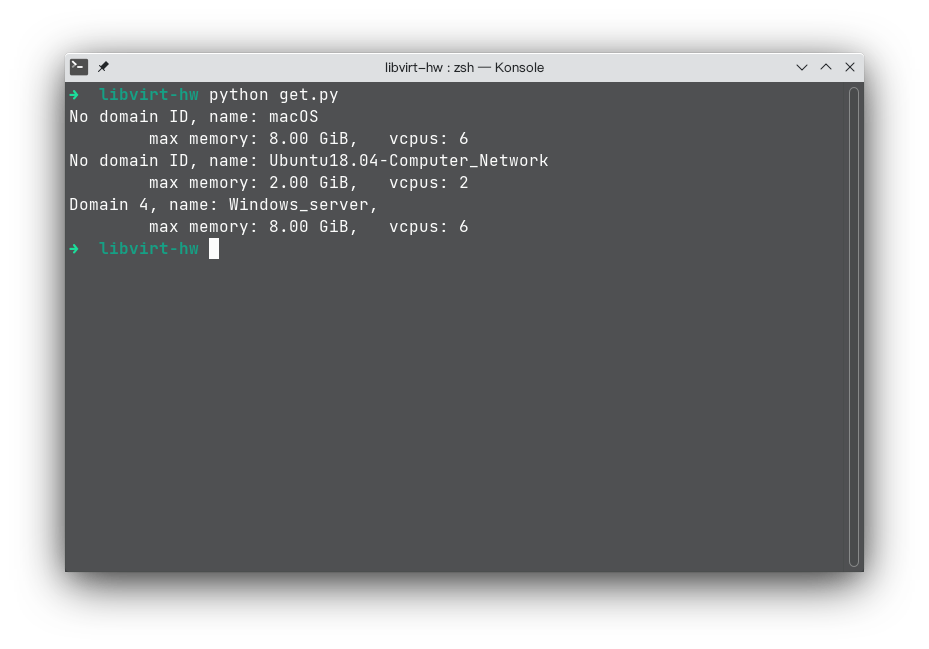
\includegraphics[width=\textwidth]{fig1.png}
    \caption{Running figure}
    \label{fig:f}
\end{figure}

The infomation can also be retrieved by \texttt{getAllDomainStats(self)}. Below is an example output of this. It will return a list of tuples of \texttt{virDomain} object instance and state dictionary.

\begin{lstlisting}[language=python]
In [28]: connection.getAllDomainStats()
Out[28]: 
[ ...
 (<libvirt.virDomain at 0x7fbd03d72e80>,
  {'state.state': 1,
   'state.reason': 1,
   'cpu.time': 455619378195086,
   'cpu.user': 31038340000000,
   'cpu.system': 126245920000000,
   'cpu.cache.monitor.count': 0,
   'balloon.current': 8388608,
   'balloon.maximum': 8388608,
   'balloon.last-update': 1637821728,
   'balloon.rss': 8384580,
   'vcpu.current': 6,
   'vcpu.maximum': 6,
   'vcpu.0.state': 1,
   'vcpu.0.time': 132681480000000,
   'vcpu.0.wait': 0,
   ...
   'net.count': 1,
   'net.0.name': 'vnet3',
   'net.0.rx.bytes': 10516726405,
   'net.0.rx.pkts': 9178957,
   'net.0.rx.errs': 0,
   'net.0.rx.drop': 0,
   'net.0.tx.bytes': 412334634,
   'net.0.tx.pkts': 1963818,
   'net.0.tx.errs': 0,
   'net.0.tx.drop': 0,
   'block.count': 1,
   'block.0.name': 'sda',
   ...})]
\end{lstlisting}

The memory can be retrieved as \texttt{balloon.} entries, as virtIO uses balloon model to abstract the memory. Other information can also be retrieved by using \texttt{virDomain}'s attributes.

\newpage

\section{Code}

The code is shown below.\footnote{This can be downloaded  \textcolor{blue}{\href{https://gist.github.com/Victrid/c7cb3ee702c6c32d31f7c1915c7cd972}{here}}.}

\begin{lstlisting}[language=python]
import libvirt

# Connect to local

# connection = libvirt.open() # with permission

# connection = libvirt.openReadOnly() # No permission

connection = libvirt.open("qemu+ssh://victrid@192.168.1.2/system")

# This will return the current running Domains ID

# domain_list = connection.listDomainsID()

domain_list = connection.listAllDomains()

def human_readable_size(size, decimal_places=2):
    for unit in ['KiB', 'MiB', 'GiB', 'TiB', 'PiB']:
        if size < 1024.0 or unit == 'PiB':
            break
        size /= 1024.0
    return f"{size:.{decimal_places}f} {unit}"

for domain in domain_list:
    id = domain.ID()
    name = domain.name()
    _, max_mem, _, nvcpu, _ = domain.info()
    if id == -1:
    # Only running domain can get domain.id
        print("No domain ID, name: {}\n\tmax memory: {},\tvcpus: {}"
            .format(name, human_readable_size(max_mem), nvcpu))
    else:
        print("Domain {}, name: {},\n\tmax memory: {},\tvcpus: {}"
            .format(id, name, human_readable_size(max_mem), nvcpu))
\end{lstlisting}

\section{Conclusion}

\emph{omitted}
\end{document}
